\chapter{Introduction}
\label{cha:intro}

%The patent system is designed to encourage disclosure of new technologies and novel ideas by granting exclusive rights on the use of inventions to their inventors, for a limited period of time. An important requirement for a patent to be granted is that the invention, it describes, is novel which means there is no earlier patent, publication or public communication of a similar idea. To ensure the novelty of an invention, patent offices as well as other Intellectual Property (IP) service providers perform searches called `prior art searches' or `validity searches'. Since the number of patents in a company's patent portfolio affects the company market value, well-performed prior art searches are of high importance~\citep{piroi2013overview}.\\\\
%\noindent
%\textbf{Patent Retrieval }
%\ \\
%Evaluation of patent retrieval was proposed in NTCIR-2 in 2001~\citep{leong2001patent}. Since then patent retrieval has featured as a track in all NTCIR campaigns. The \emph{Clef-Ip Lab} and its tasks have evolved considerably over the last five years, from a rough approximation of a prior art search task in 2009, to, in 2013, a good simulation of the passage-level search carried out by patent searchers~\citep{piroi2013passage}. Patent retrieval is of interest in IR research since it is of commercial interest and is a challenging IR task with different characteristics to popular IR tasks such as precision-orientated ad hoc search on news archives or web document collections. Various patent search tasks have been created in mentioned campaigns including:
%\\
%\textbf{\textit{Ad-hoc search:}} A number of topics are used to search a patent collection with the objective of retrieving a ranked list of patents that are relevant to this topic~\citep{iwayama2003overview}.\\\\
%\textbf{\textit{Invalidity search.}} The claims of a patent are considered as the topics, and the objective is to search for all relevant documents (patents and others) to find whether the claim is novel or not~\citep{joho2010survey, fujii2004overview}. All relevant documents are needed, since missing only one document can lead to later invalidation of the claim or the patent itself.
%\\\\
%\textbf{\textit{Passage Search:}} The same as invalidity search, but because patents are usually long,
%the task focuses on indicating the important fragments in the relevant documents~\citep{fujii2007overview}.\\\\
%\textbf{\textit{Prior-art Search:}}
%This is the main search task carried out in patent offices; it is concerned with finding all relevant patents that are potential to invalidate the novelty of a patent application or at least that have common parts to that patent~\citep{roda2010clef}. The full patent application submitted to the patent office is considered as the topic, and patent citations that are identified by the patent office are taken as the relevant documents, therefore the objective is to find these citations of patents automatically. Prior-art search in patent retrieval focuses on finding any kind of patents relevant to the patent application in hand; this is different from invalidity search which focuses on finding any type of document that proves that a given claim in a patent application is not novel.\\\\
%\textbf{Main challenges of prior-art search}
%\\ \
%\textit{\textbf{Query length:}} The query is a full patent application instead of just keywords which are short. So it is not focused on information need. The problem with a full document as a query is that, it might refer to multiple topics. Even in the case of a single invention, different components of the new device or process which may be described in verbose patent application. \\\\
%\textit{\textbf{Recall-oriented retrieval task:}} Prior-art search is a recall-oriented retrieval task, where not missing a relevant document is more important than retrieving a small number of the most relevant documents at the top rank. Usually, in prior-art search, the patent examiners will carefully examine the first 100 or 200 documents retrieved by the search engine instead of browsing just the top few results. Missing one patent could result in a multimillion dollar lawsuit due to a patent infringement~\citep{arampatzis2007access, magdy2010pres}. \\\\
%\textit{\textbf{Term Mismatch: }} The biggest challenge in patent retrieval is the significant term mismatch between the query and relevant document (Due to: Usage of new inventive words, Rewording to avoid repetition, Non-standardized acronyms: invented by authors, Synonyms: signal and wave). Magdy~\citep{magdy2010exploring} reported from their analysis presented for CLEF-IP 2009 prior-art search that 12\% of the relevant patents do not share any terms in common with patent topics after filtering out stop words ~\citep{magdy2011study}.
%\begin{figure}[htpb]
%   \centering
%   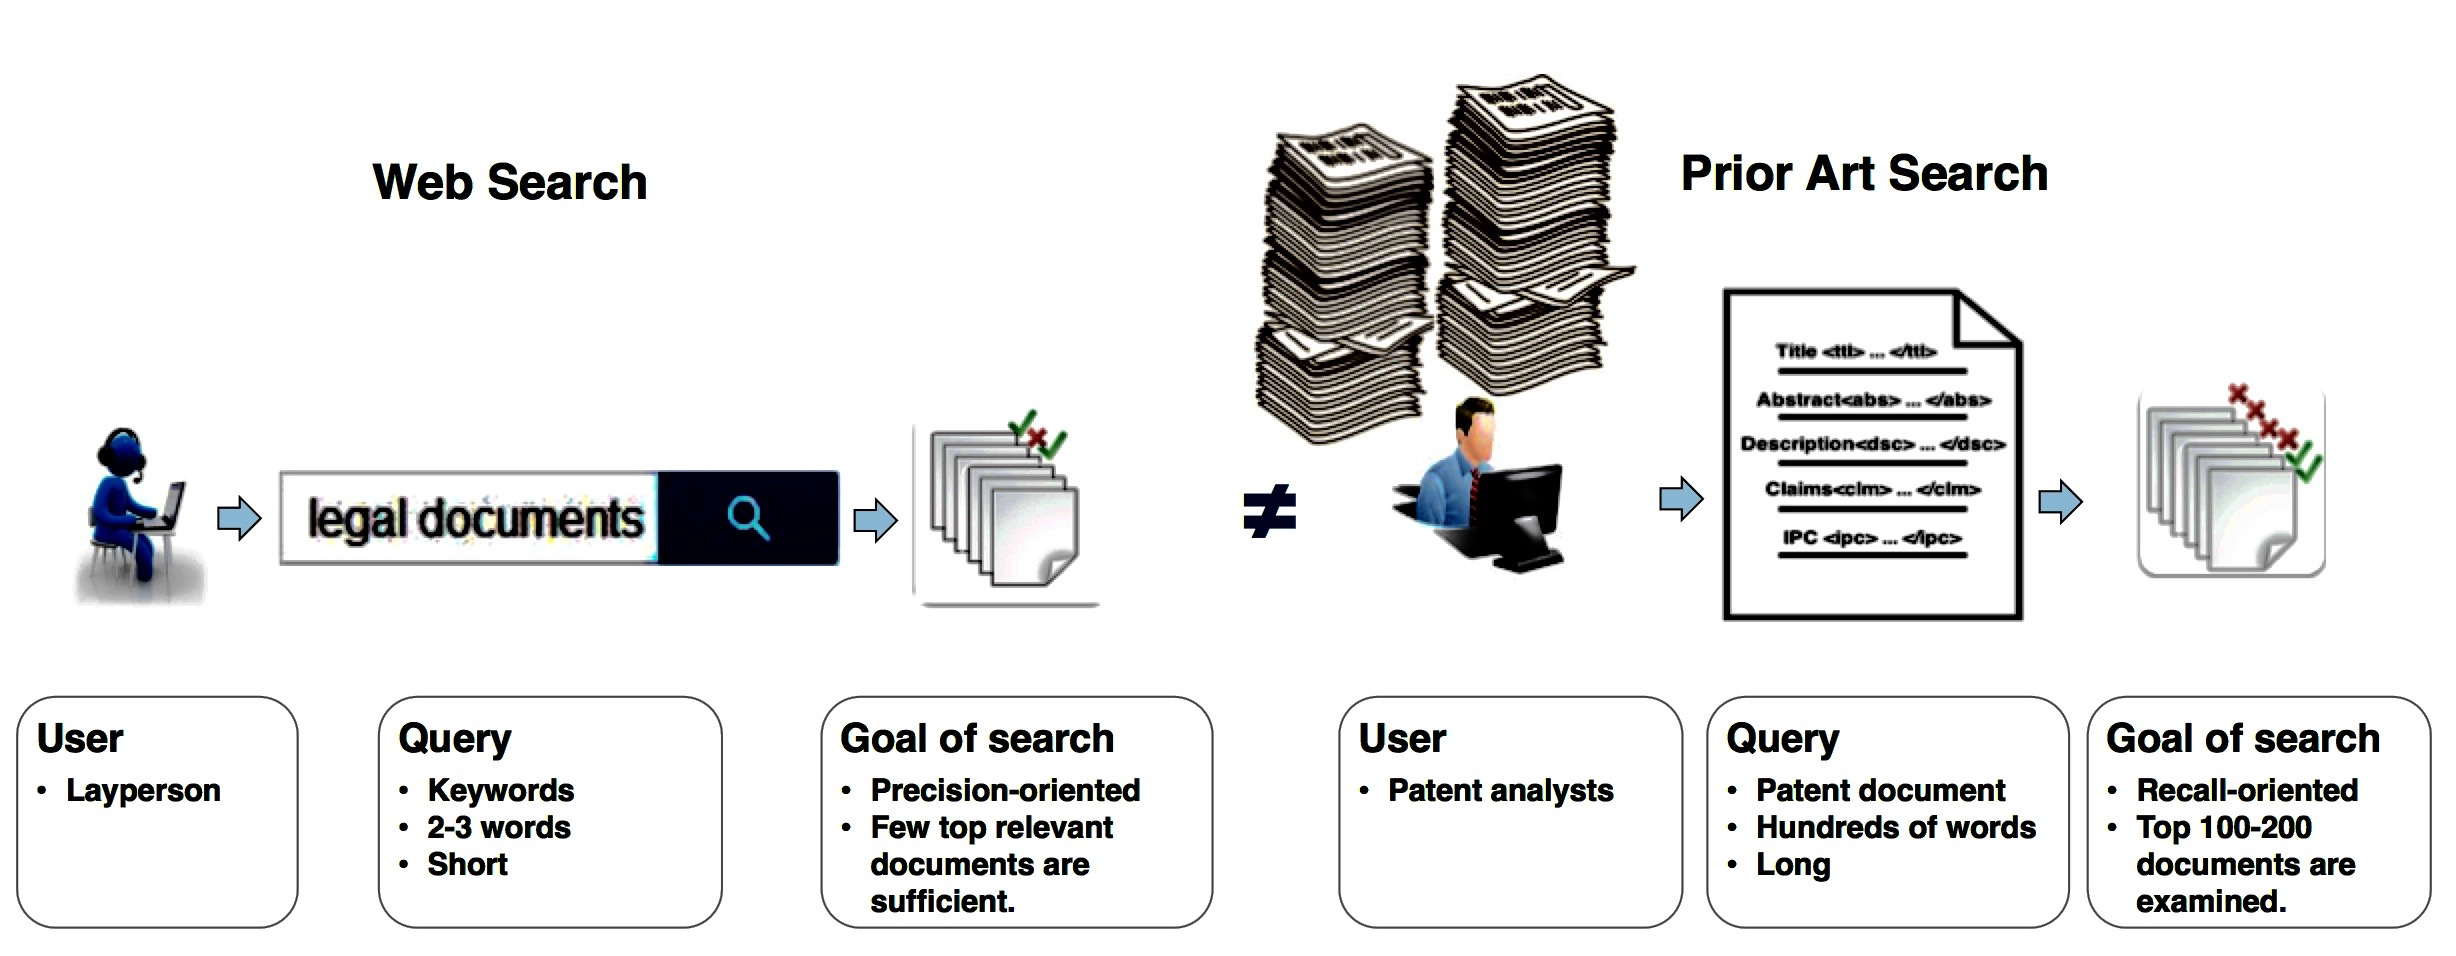
\includegraphics[width=\textwidth,height=35mm]{figs/webprior.jpg}
%   \caption{The main differences between patent prior-art search and an standard web search are: (1) the user is an expert (professional patent examiner), (2) the query is a full application not just keywords, and (3) it is a recall oriented task.}  
%   \label{fig:compareappr} 
%\end{figure}
%\FloatBarrier 
%\noindent
%\textbf{Problem Statement :}
%Applying standard information retrieval (IR) techniques to patent search is not effective and needs applying supplementary methods to improve its effectiveness. Although lots of methods has been proposed in recent years but still reported results for different tasks of patent search show lower retrieval effectiveness compared to other IR applications \citep{lupu2013patent}. For example, it is generally expected to achieve a mean average precision (MAP) less than 0.1, which is still regarded as an acceptable level of effectiveness. The results of various evaluation campaigns ~\citep{lupu2013patent,joho2010survey, roda2010clef, DBLP:conf/clef/PiroiLHSMF12} concluded that patent search task is certainly not a solved problem and many challenges in applying IR solutions in the intellectual property domain remain to be overcome. In this research, we focus on enhancing possible general and patent-specific IR techniques to improve the effectiveness of baseline patent prior-art search. 
%\newpage

%%%%%%%%%%%%%%%%%%%%%%%%%%%%%%%%%%%%%%%%%%%%%%%%%%%%%%%%%%%%%%%%%%%%%%%%%%%%%%%%%%%
%\textcolor{red}{Mona: I am working on the introduction section, suggestions welcome!}
%%%%%%%%%%%%%%%%%%%%%%%%%%%%%%%%%%%%%%%%%%%%%%%%%%%%%%%%%%%%%%%%%%%%%%
\begin{figure}[htpb]
   \centering
   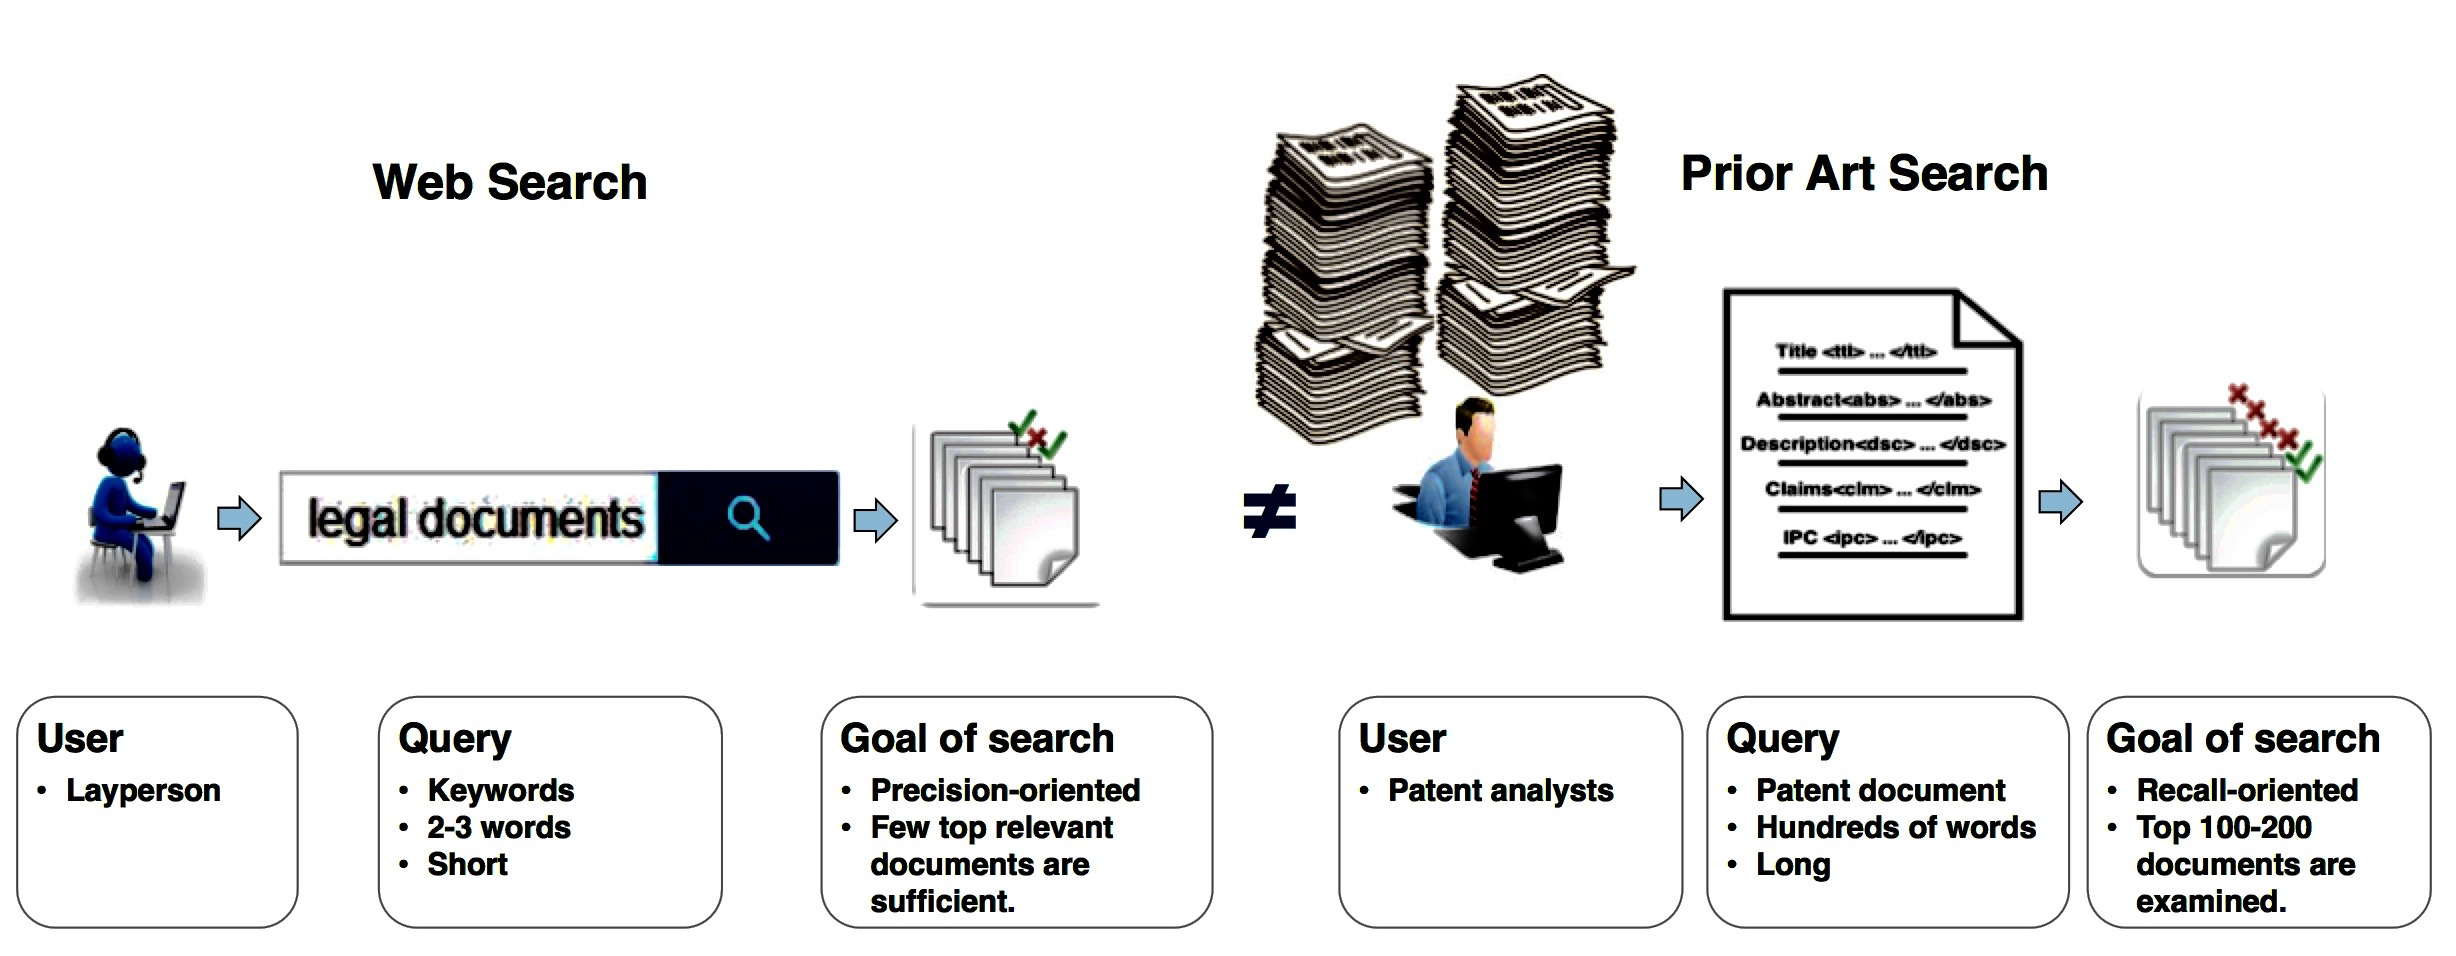
\includegraphics[width=\textwidth,height=35mm]{figs/webprior.jpg}
   \caption{The main differences between patent prior art search and an standard web search are: (i) queries are reference patent
applications, and (ii) patent prior art search is a recall-oriented task.}  
   \label{fig:compareappr} 
\end{figure}
\FloatBarrier
%%%%%%%%%%%%%%%%%%%%%%%%%%%%%%%%%%%%%%%%%%%%%%%%%%%%%%%%%%%%%%%%%%%%%%
\section{Motivation}
\label{sec:Motivation}
Patent prior art search involves finding previously granted patents,
or any published work, such as scientific articles or product
descriptions that may be relevant to a new patent application. 
The objective and challenges of standard formulations of patent prior art
search are different from those of standard text and web search~\citep{magdy2012toward}.

The main characteristic of prior art search is that queries are reference patent
applications, which consist of documents with hundreds or thousands of
words organised into several sections, while typical queries in text
and web search constitute only a few words. 
In addition, in contrast to scientific and technical writers, patent writers
tend to generalise and maximise the scope of what is protected by a
patent and potentially discourage further innovation by third parties,
which further complicates the task of formulating queries. 
Searching based on patent queries helps patent examiners to save time and avoid 
formulating appropriate search queries out of long and difficult patent applications. In general, patent
examiners spend about 12 hours to complete an invalidity task by examining
approximately 100 patent documents retrieved by 15 different queries in average~\citep{joho2010survey}.

Another important characteristic of patent prior art
search is being a recall-oriented task, where the primary focus is to
retrieve all relevant documents at early ranks, in contrast to text
and web search that are precision-oriented, where the primary goal is
to retrieve a subset of documents that best satisfy the query
intent (according to~\citep{zhang2010search}, 44.5\% of web search users examine only one retrieved document). 
In prior art search, missing relevant documents is unacceptable because of the highly commercial nature of patents coupled with the high costs involved
in creating a patent and infringing patented material~\citep{joho2010survey}.

The main users of patent prior art search are 
patent analysts, who are employed to determine the patentability 
of applications. We do not consider inventors, who want to determine whether their ideas are novel, as users of patent prior art search, because the prior art search starts with querying by a patent application that is not written when the author is going to check its novelty.
Patent searchers have to perform an exhaustive and comprehensive search.

Users can save time if they start searching for prior art with a patent document as a query. However, this approach is less effective than web search
~\citep{lupu2013patent}. In this thesis, we study query reformulation to transform an initial query (i.e., patent document) to another query to improve retrieval effectiveness. We mainly emphasise on query term selection techniques to formulate a query, which achieves the highest performance.

%in formulating an effective query, we study 
%the query term selection techniques and the sufficiency of 
%terms in the reference patent queries resulting in an improved 
%retrieval performance.   

\section{Summary}
\label{sec:summary}
In this work, we focus on the task of query
reformulation~\citep{Baeza-Yates2011} specifically applied to patent
prior art
search~\citep{mahdabi2014patent,Piroi2010,xue2009transforming}. While
prior work has largely focused on specific techniques for query
reformulation, 
%in Section \ref{Sec:OracularTermSelection}
 we first
build an oracular query formed from known relevance judgments for the
CLEP-IP 2010 Prior Art test collection~\citep{Piroi2010} in an attempt
to derive an upper bound on performance of standard Okapi BM25 and
Language Models (LM) retrieval algorithms for this task.  Since the
results of this evaluation suggest that query reduction methods can
outperform state-of-the-art prior art search performance, 
%in Section \ref{sec:AutomatedReduction} 
we proceed to analyze four simple
automated methods for identifying terms to remove from the original
patent query.  Finding that none of these methods seems to
independently yield promise for query reduction that strongly
outperforms the baseline, 
%in Section \ref{sec:SemiAutomatedInteractiveReduction} 
we evaluate an alternative
interactive feedback approach where terms are selected from only the
first retrieved relevant document.  Observing that such simple
interactive methods for query reduction with a standard LM retrieval
model outperform highly engineered patent-specific search systems from
CLEF-IP 2010, we conclude that interactive methods offer a promising
avenue for simple but highly effective term selection in patent prior
art search.

\section{Contributions}
\label{sec:Contributions}
This thesis proposes term selection techniques for patent prior art search.
%exact optimal solutions to H-MDP and H-POMDP, working
%around some of the limitations of previous approaches. 
The main contributions of this work are summarized as follows:
\begin{itemize}
\item We developed an oracular relevance feedback system which extracts terms from the judged relevant documents that far outperformed the the baseline and around twice as well on MAP as the best competitor in CLEF-IP 2010. Experiments related to oracular system suggests the necessity of precise query reduction and term selection techniques to improve the effectiveness for patent prior art search.
\item We examined four simple query reduction methods to select useful words and prune out noisy words. We illustrated that these approaches are inefficient because they cannot discriminate between useful and noisy words. Since our system is over-sensitive to the existence of noisy words, we could not achieve high performance via these simple methods.
\item We showed that a simple minimal interactive relevance feedback approach can perform as well as a highly engineered patent specific search system for CLEF-IP 2010.
\end{itemize}
\section{Thesis Outline}
\label{sec:outline}
The rest of the thesis is organised as follows: Chapter ~\ref{cha:background} reviews previous work from a number
of related research areas, and Chapter~\ref{cha:BaselineIRFramework} describes baseline and experimental Settings, 
test collections (i.e., queries and relevance judgments),
etc. In Chapter~\ref{cha:BaselineIRFramework}, we also describe data curation and IPC filter errors.
Chapter~\ref{cha:analysis} contains the discussion and results related to our main analysis, where we figure out 
the main cause of low effectiveness of prior art search and then we propose and test the possible term selection methods. 
%we propose our query generation frameworks,
%suggestion methods, and diversification approaches; Chapter 4, Chapter 5, Chapter 6,
%and Chapter 7 describes Boolean query generation, phrasal-concept query generation,
%diverse query generation, and search result diversification, respectively. In each of
%these chapters, 
%we provide experimental results and relevant discussion. 
In Chapter~\ref{cha:conc}, we finally conclude this thesis by 
summarising the results and discussing future work.


%How many chapters you have? You may have Chapter~\ref{cha:background},
%Chapter~\ref{cha:design}, Chapter~\ref{cha:methodology},
%Chapter~\ref{cha:result}, and Chapter~\ref{cha:conc}.
